% !TEX root = ./thesis.tex
\subsection{Effects of Filtering in a Well-resolved Simulation}
\label{sec:filteringEffects}

This Section shows that the use of \gls{lfs} has effects similar to using artificial viscosity. The previous results show that \gls{lfs} filters can stabilize even the most extreme of circumstances. What about the effect of using \gls{lfs} filters in more reasonable conditions?

The case of 2-D flow over a circular cylinder at \gls{re} $=3,900$, \gls{ma} $=0.1$ has been selected given the good amount of computational results for it. The thesis by Beaudan \cite{beaudan1994numerical} provides a very thorough discussion of the physics of the 3-D problem and results of simulations with structured high-order methods.

At \gls{re} $=3,900$, a proper simulation of flow around a circular cylinder must be 3-D \cite{breuer1998large}. In fact, previous 2-D simulations of this case have shown the flow to be highly asymmetric \cite{breuer1998large}. The aim of the simulations presented here is not to predict experimental results, but rather to provide an understanding of how the flow will be affected by the use of \gls{lfs} filters. We will see that the \gls{lfs} filters act as artificial viscosity: flow that would otherwise exhibit chaotic behavior becomes periodic. A similar transition from chaotic to periodic behavior due to added dissipation (via turbulence modeling) has been observed in \gls{urans} simulations \cite{catalano2003numerical}.

\subsubsection{Setup}
\label{sec:filterEffectsSetup}

We first generate a grid for a $2^{\mathrm{nd}}$ order method that resolves the $y+$ scales around the cylinder. We then generate grids that maintain close to the same number of \gls{dof} for a \nth{5}  and \nth{6} spatial order of accuracy scheme. We perform the simulation of \gls{re}$=3.9e3$ past a circular cylinder using the \nth{5} and \nth{6} order schemes in the different grids. The aims of this setup are to:
\begin{enumerate}
\item Have a well-resolved, baseline case
\item Visualize the effects of changing the spatial order of accuracy while maintaining the number of \gls{dof} almost constant
\item Visualize the effects of using an under-resolved grid
\item Visualize the effects of using \gls{lfs} filters in different grids with different spatial orders of accuracy
\end{enumerate}

A baseline case with a \nth{6} order accurate in space scheme was attempted while maintaining the same number of degrees of freedom as the case with the $2^{\mathrm{nd}}$ order scheme. However, the non-linearities within the relatively large elements elements prevented the simulation from completing without intervention. However, a simulation with filtering in the same grid with the same order of accuracy did run to completion.

In addition, to compare the effects of filtering versus running a slightly unresolved simulation, an unfiltered case of a slightly unresolved grid was run with a \nth{5} order scheme.

Finally, a well resolved, yet filtered, simulation with the \nth{5} order scheme was performed.

All cases ran with the same non-dimensional time-step of $\Delta t = 1e-5$ for a non-dimensional time of $t = 64.7$. Given that \gls{ma} $=0.1$, temperature of air simulated was $300K$, $\gamma = 1.4$, and the reference length was $1$ meter, the physical time-step was $2.88e-6$ seconds and the physical simulation time was $1.86$ seconds.

Filtering is performed with a value of $h = 10$ in Equation \eqref{eq:sharp_spectral} and $\alpha = 0.8$ in Equation \eqref{eqn:filter_form}. All conservation fields are filtered every 500 time-steps, so every $5e-2$ non-dimensional time units, or every $1.44e-3$ seconds. The filtering procedure was kept the same to isolate the effects of filtering. In practice, a sensor should be used in order to only filter the elements where instabilities could arise.


\subsubsection{Results and Discussion}
\label{sec:filterEffectsResults}

Table \ref{table:filteringEffect_simSummary} summarizes all the cases run and provides hyperlinks to videos of the resulting flow simulations. The value of \gls{st} provided reflects the peak \gls{st} of the lift coefficient power spectrum.

All cases display the following phases: a pair of vortices strengthen behind the cylinder, the vortices elongate and the drag coefficient decreases, asymmetries in the solution trigger vortex shedding, the vortex growth and shedding process transitions into a quasiperiodic (when not filtered) or periodic (when filtered) behavior.

\begin{table}
%\begin{adjustwidth}{-2.1cm}{}
%    \centering
\cellspacebottomlimit=5pt
\cellspacetoplimit=5pt
%      \begin{center}                % keep track of old \tabcolsep
\setlength{\oldtabcolsep}{\tabcolsep}     % 6.0pt
\setlength{\tabcolsep}{0pt}               % so coloring doesn't run off
% ends of the table
\renewcommand{\arraystretch}{2}         % because math expressions
% almost run into each other

\def \spacing {0.4cm}
\hspace{-0.5cm}
\begin{tabular}{c <{\hspace{\len}} c <{\hspace{\len}} c <{\hspace{\len}} c <{\hspace{\spacing}} 
c <{\hspace{\spacing}}
c<{\hspace{\spacing}} c<{\hspace{\spacing}} c<{\hspace{\spacing}} c}
\toprule
Case & $P$  & Mesh & Filtered & Grid & $\#$ \gls{dof} & \specialcell[b]{$C_L$ and $C_D$ vs. $t$ \vspace{-0.2cm}\\Figure}   &  \specialcell[b]{\gls{st}} & \specialcell[b]{Video} \\
\specialrule{\lightrulewidth}{0pt}{0pt} % so row-coloring aligns

\hypertarget{caseA}{A} & 1 &  \ref{fig:mesh_case_A} & No & \ref{fig:mesh_case_A} & 1,579,620 & \ref{fig:history_P1_noFilt_mesh1} & 0.19 & \href{https://www.youtube.com/watch?v=mtUrv-Aj_y0}{link} \\
\hypertarget{caseB}{B} & 4 & \ref{fig:mesh_case_BDG} & No & \ref{fig:mesh_case_BDG} & 1,398,780 & \ref{fig:history_P4_noFilt_mesh4} & 0.17 & \href{https://www.youtube.com/watch?v=FpyAf08kz7A}{link} \\
\hypertarget{caseC}{C} & 4 & \ref{fig:mesh_case_C} & No & \ref{fig:mesh_case_C} & 703,260 & \ref{fig:history_P4_noFilt_mesh6} & 0.17 & \href{https://www.youtube.com/watch?v=Tud7N1tmmrA}{link} \\
\hypertarget{caseD}{D} & 4 & \ref{fig:mesh_case_BDG} & Yes & \ref{fig:mesh_case_BDG} & 1,398,780 & \ref{fig:history_P4_filt_mesh4} & 0.25 & \href{https://youtu.be/H1xKenZ2g6Q}{link} \\
\hypertarget{caseE}{E} & 5 & \ref{fig:mesh_case_EF} & No & \ref{fig:mesh_case_EF} & 1,362,396 & Unstable & N/A & N/A \\
\hypertarget{caseF}{F} & 5 & \ref{fig:mesh_case_EF} & Yes & \ref{fig:mesh_case_EF} & 1,362,396 & \ref{fig:history_P5_filt_mesh5} & 0.21 & \href{https://www.youtube.com/watch?v=FMZBi285alk}{link} \\
\hypertarget{caseG}{G} & 5 & \ref{fig:mesh_case_BDG} & Yes & \ref{fig:mesh_case_BDG} & 1,958,292 & \ref{fig:history_P5_filt_mesh4} & 0.25 & \href{https://www.youtube.com/watch?v=cmIKRwJXoME}{link} \\

\bottomrule
\end{tabular}
\caption{Simulation results that illustrate effect of filtering, changing meshes, and varying the spatial order of accuracy. All cases were run at \gls{ma} $=0.1$, \gls{re}$ = 3.9e3$.}
\label{table:filteringEffect_simSummary}
\end{table}


\begin{figure}
\centering
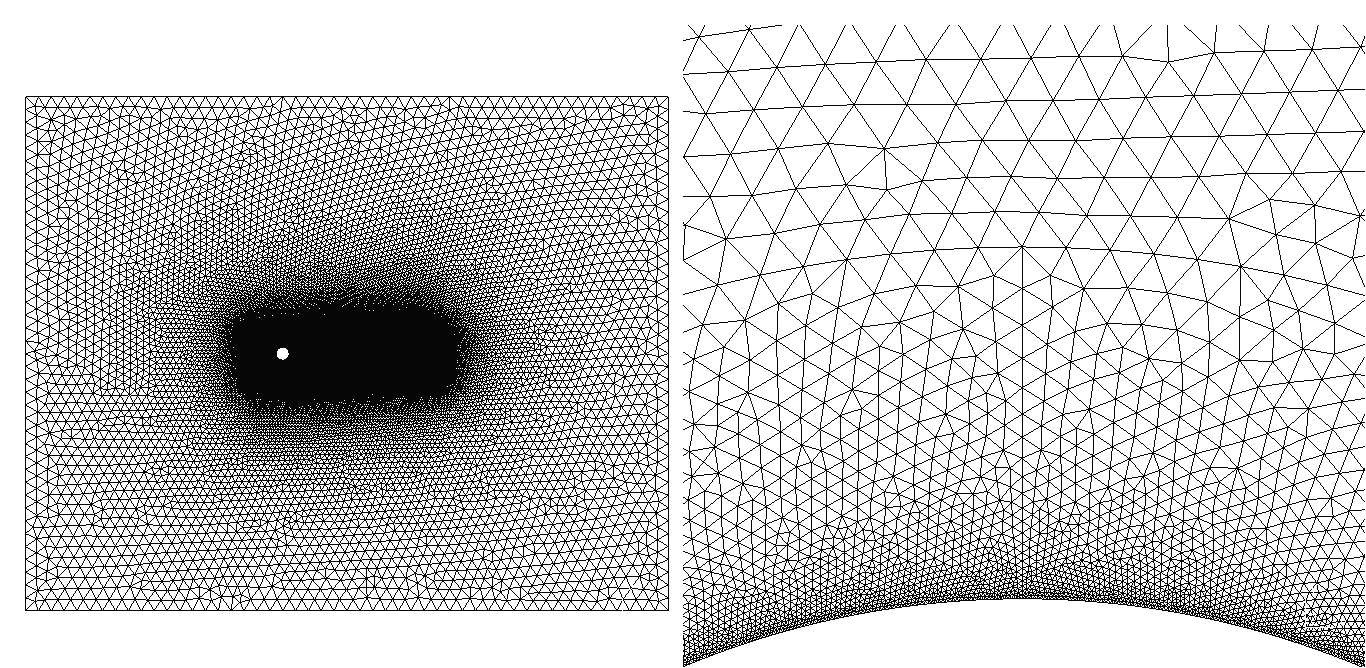
\includegraphics[width = 1\textwidth]{\lfsdir/figs/mesh_images/cylinder_1stOrder_Re3-6e3_fine1_mod.png}
\caption{Mesh used in case A in Table \ref{table:filteringEffect_simSummary}. Contains 131,635 triangular elements with second order edges.} 
\label{fig:mesh_case_A}
\end{figure}

\begin{figure}
\centering
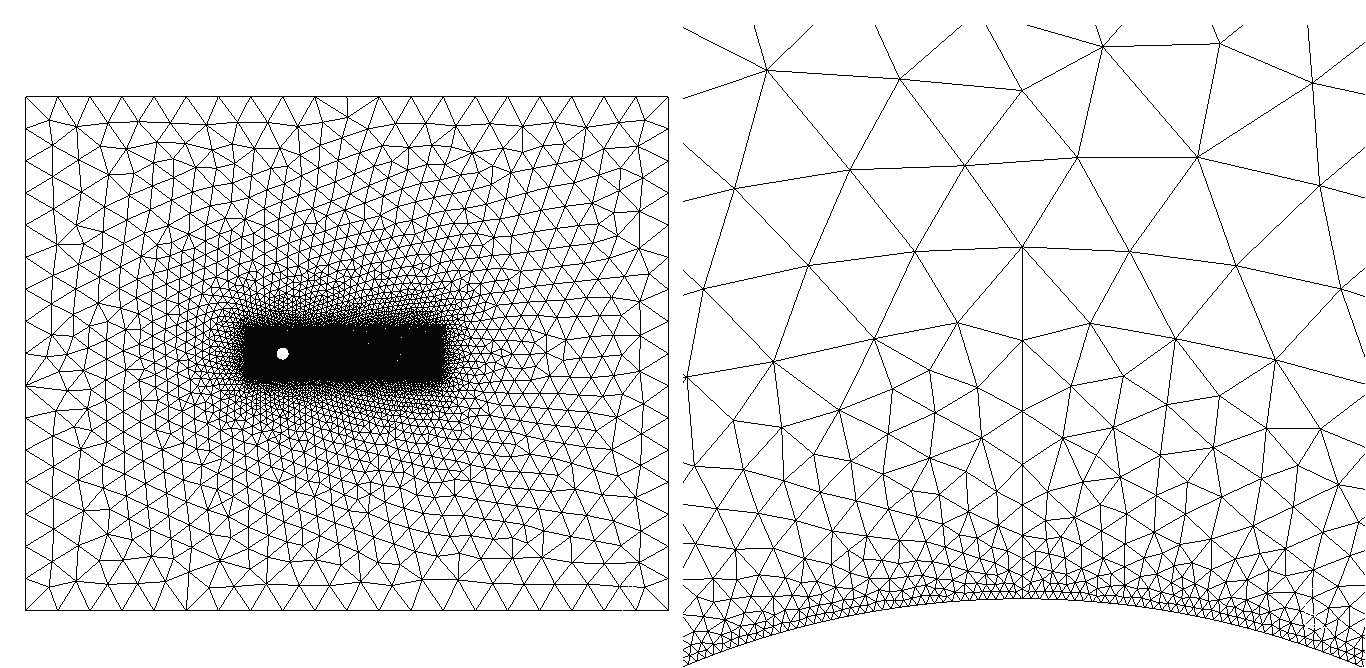
\includegraphics[width = 1\textwidth]{\lfsdir/figs/mesh_images/cylinder_4thOrder_Re3-9e3_mod.png}
\caption{Mesh used in cases B, D, and G in Table \ref{table:filteringEffect_simSummary}. Contains 23,313 triangular elements with second order edges.} 
\label{fig:mesh_case_BDG}
\end{figure}

\begin{figure}
\centering
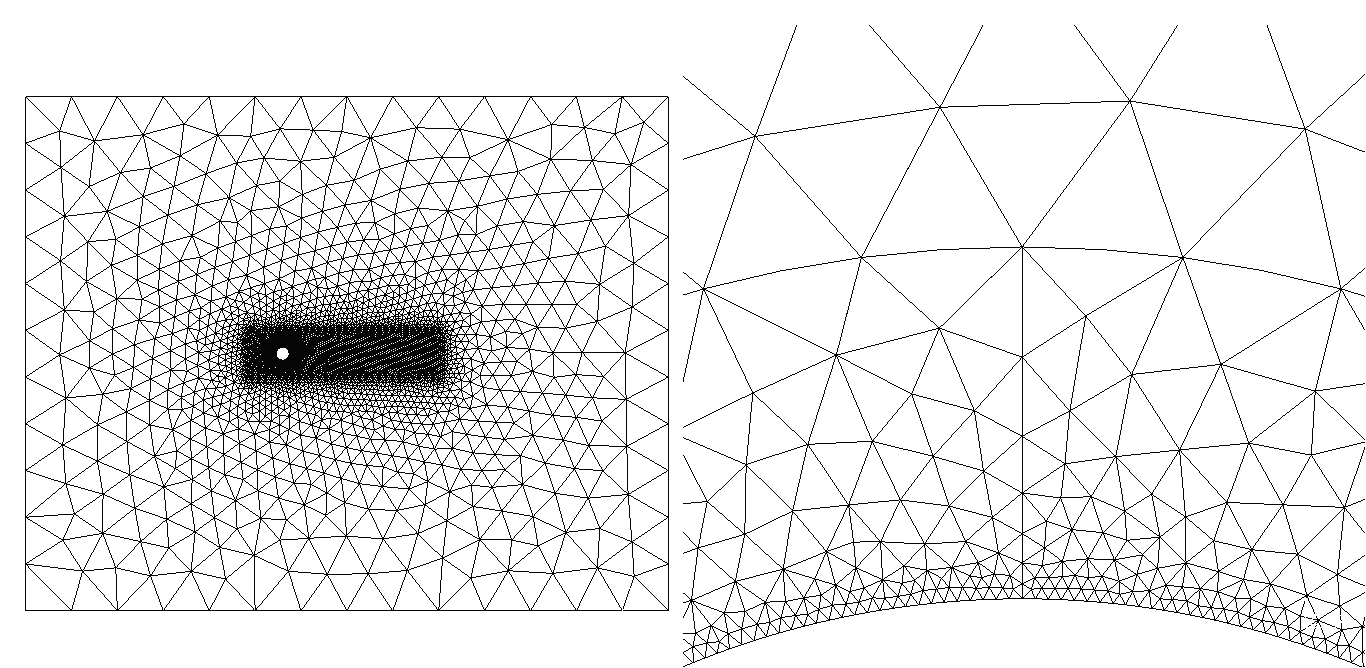
\includegraphics[width = 1\textwidth]{\lfsdir/figs/mesh_images/cylinder_6thOrder_Re3-9e3_mod.png}
\caption{Mesh used in case C in Table \ref{table:filteringEffect_simSummary}. Contains 11,721 triangular elements with second order edges.} 
\label{fig:mesh_case_C}
\end{figure}

\begin{figure}
\centering
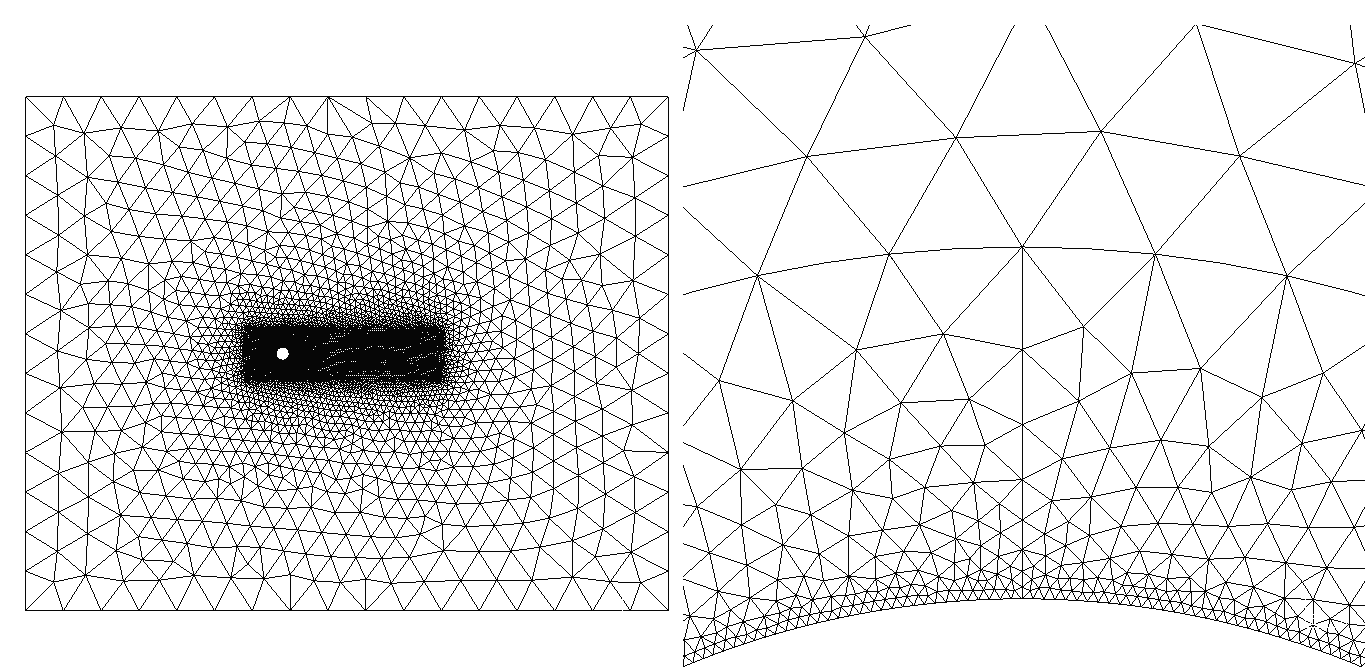
\includegraphics[width = 1\textwidth]{\lfsdir/figs/mesh_images/cylinder_5thOrder_Re3-9e3_mod.png}
\caption{Mesh used in cases E and F in Table \ref{table:filteringEffect_simSummary}. Contains 16,219 triangular elements with second order edges.}
\label{fig:mesh_case_EF}
\end{figure}

% % % % % % % % % % % % % % % % % % % % % % % %  Simulation Results

\begin{figure}
\centering
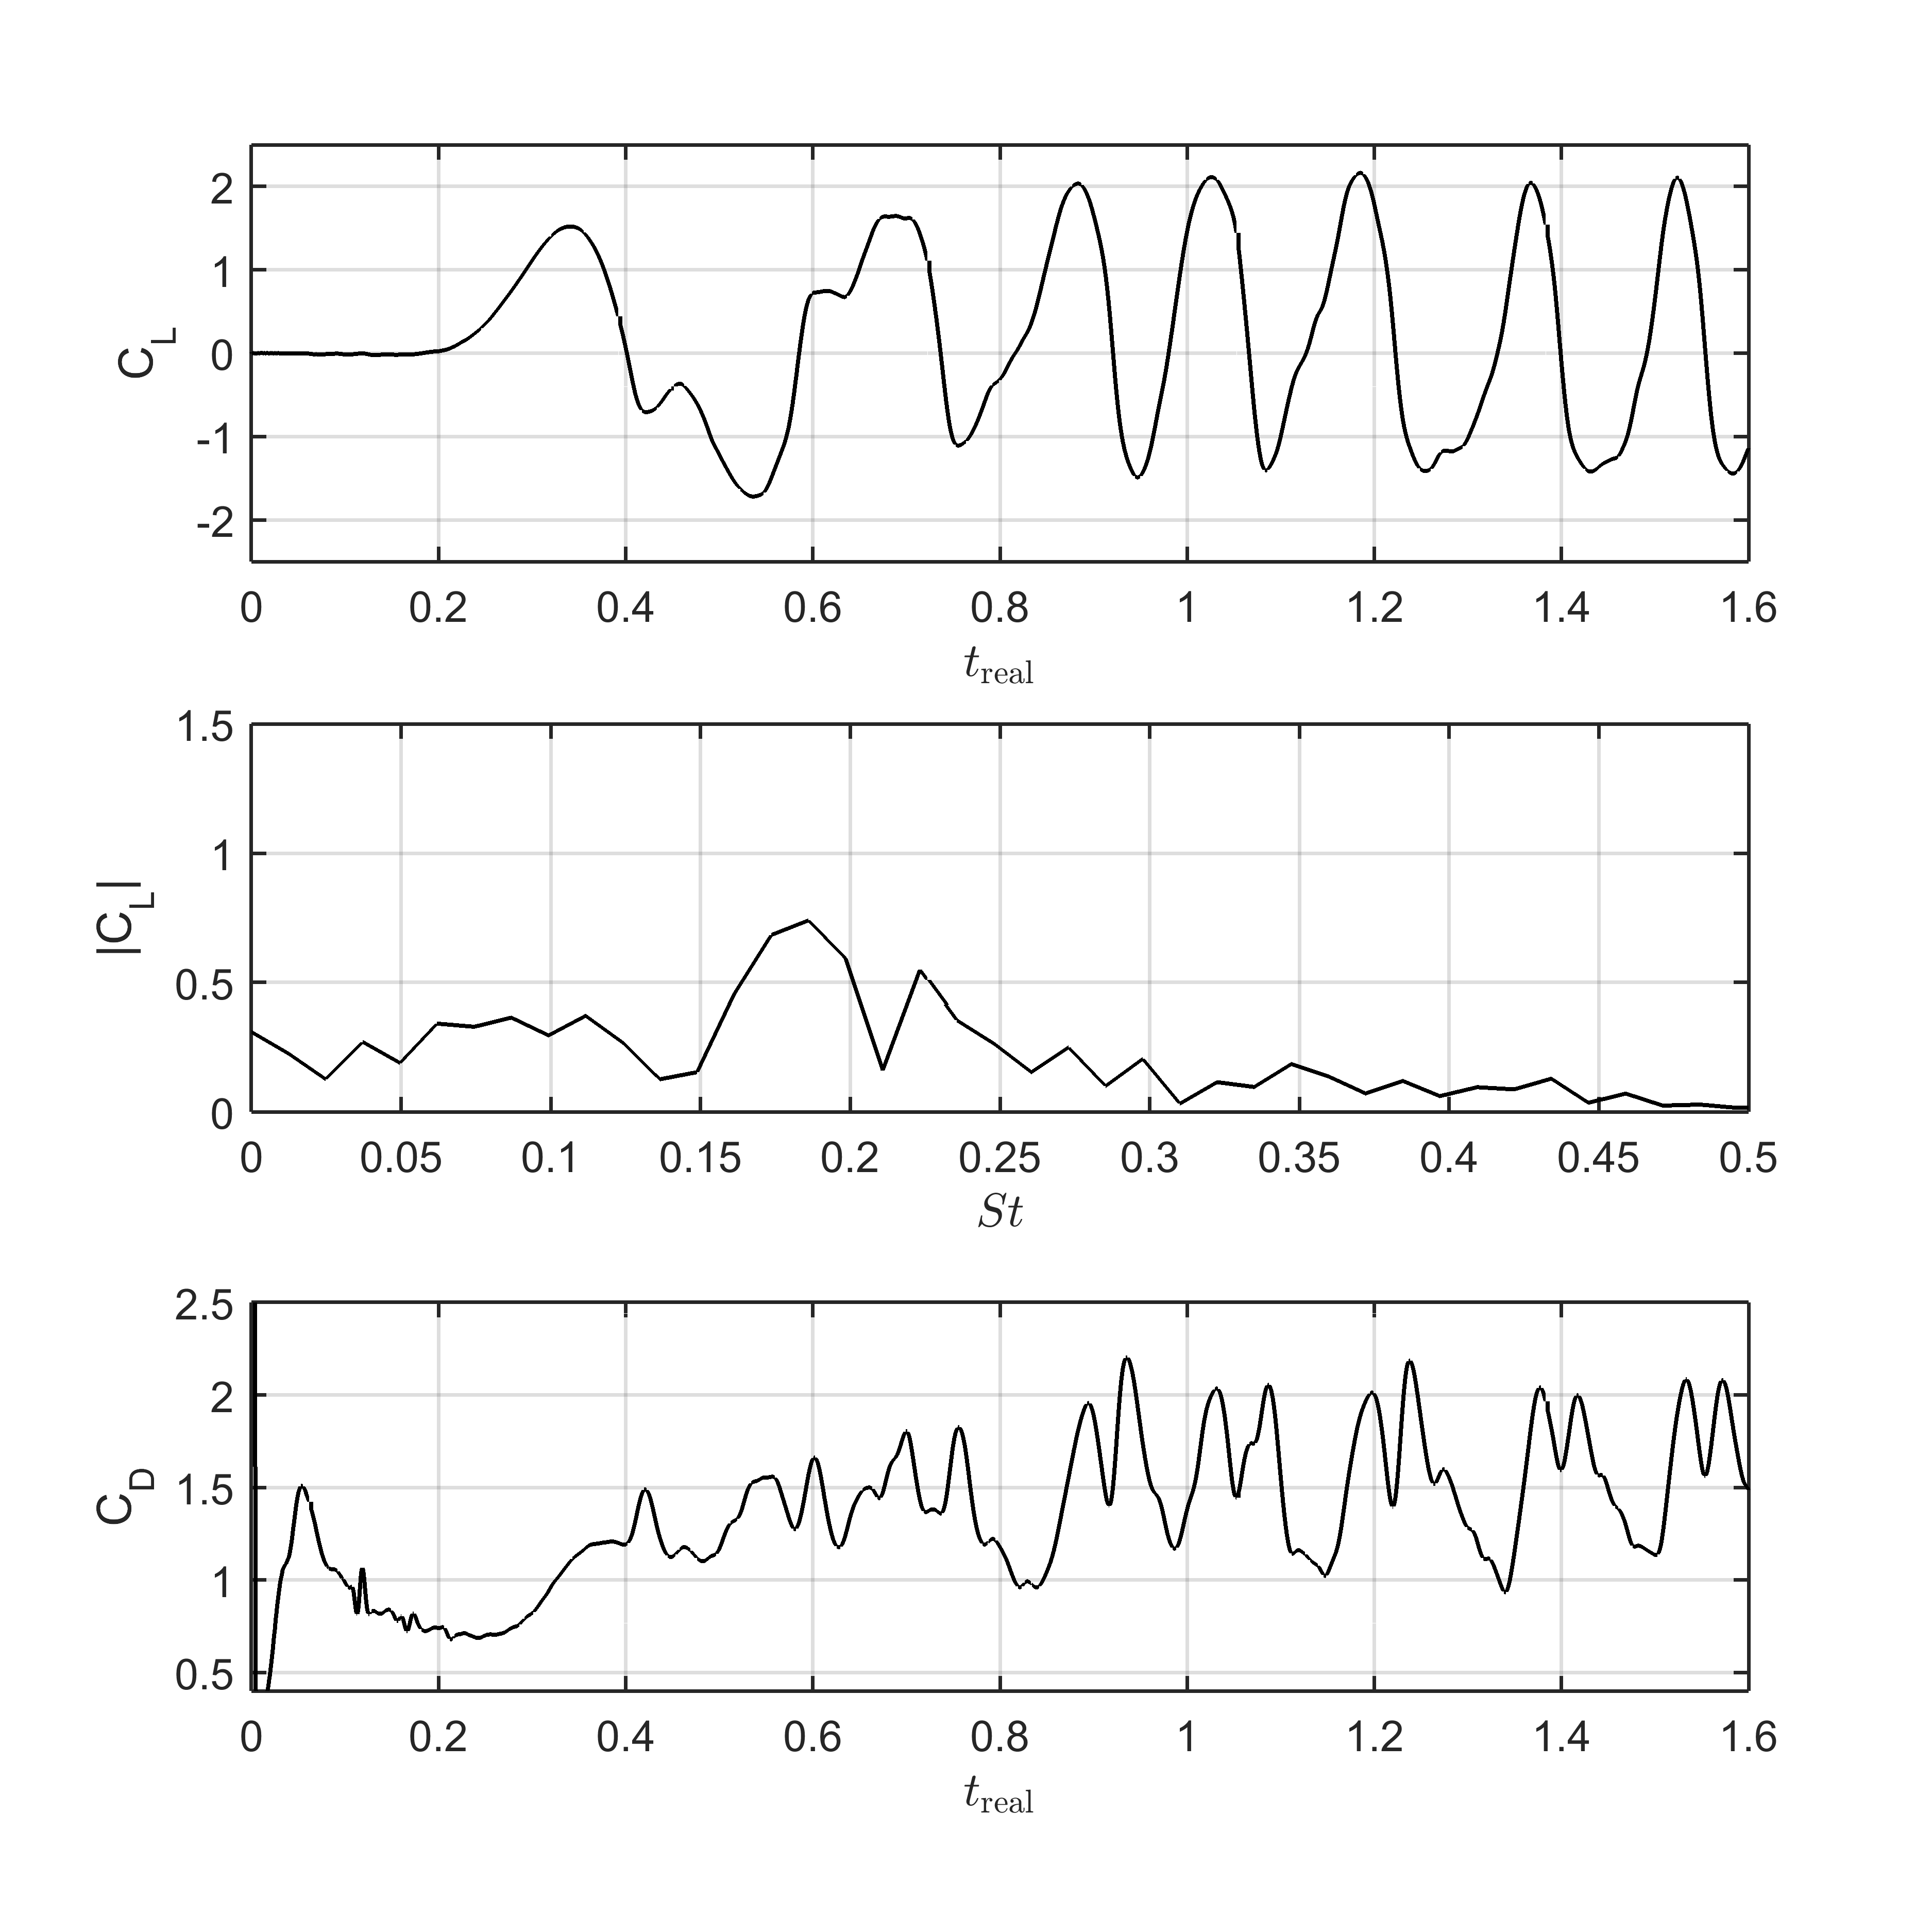
\includegraphics[width = 1\textwidth]{\lfsdir/figs/history_P1_noFilt_mesh1.png}
\caption{Case A in Table \ref{table:filteringEffect_simSummary} lift coefficient, \gls{st} power spectrum, and drag coefficient. Case is not filtered and uses mesh \ref{fig:mesh_case_A} with $P=1$. }  
\label{fig:history_P1_noFilt_mesh1}
\end{figure}

\begin{figure}
\centering
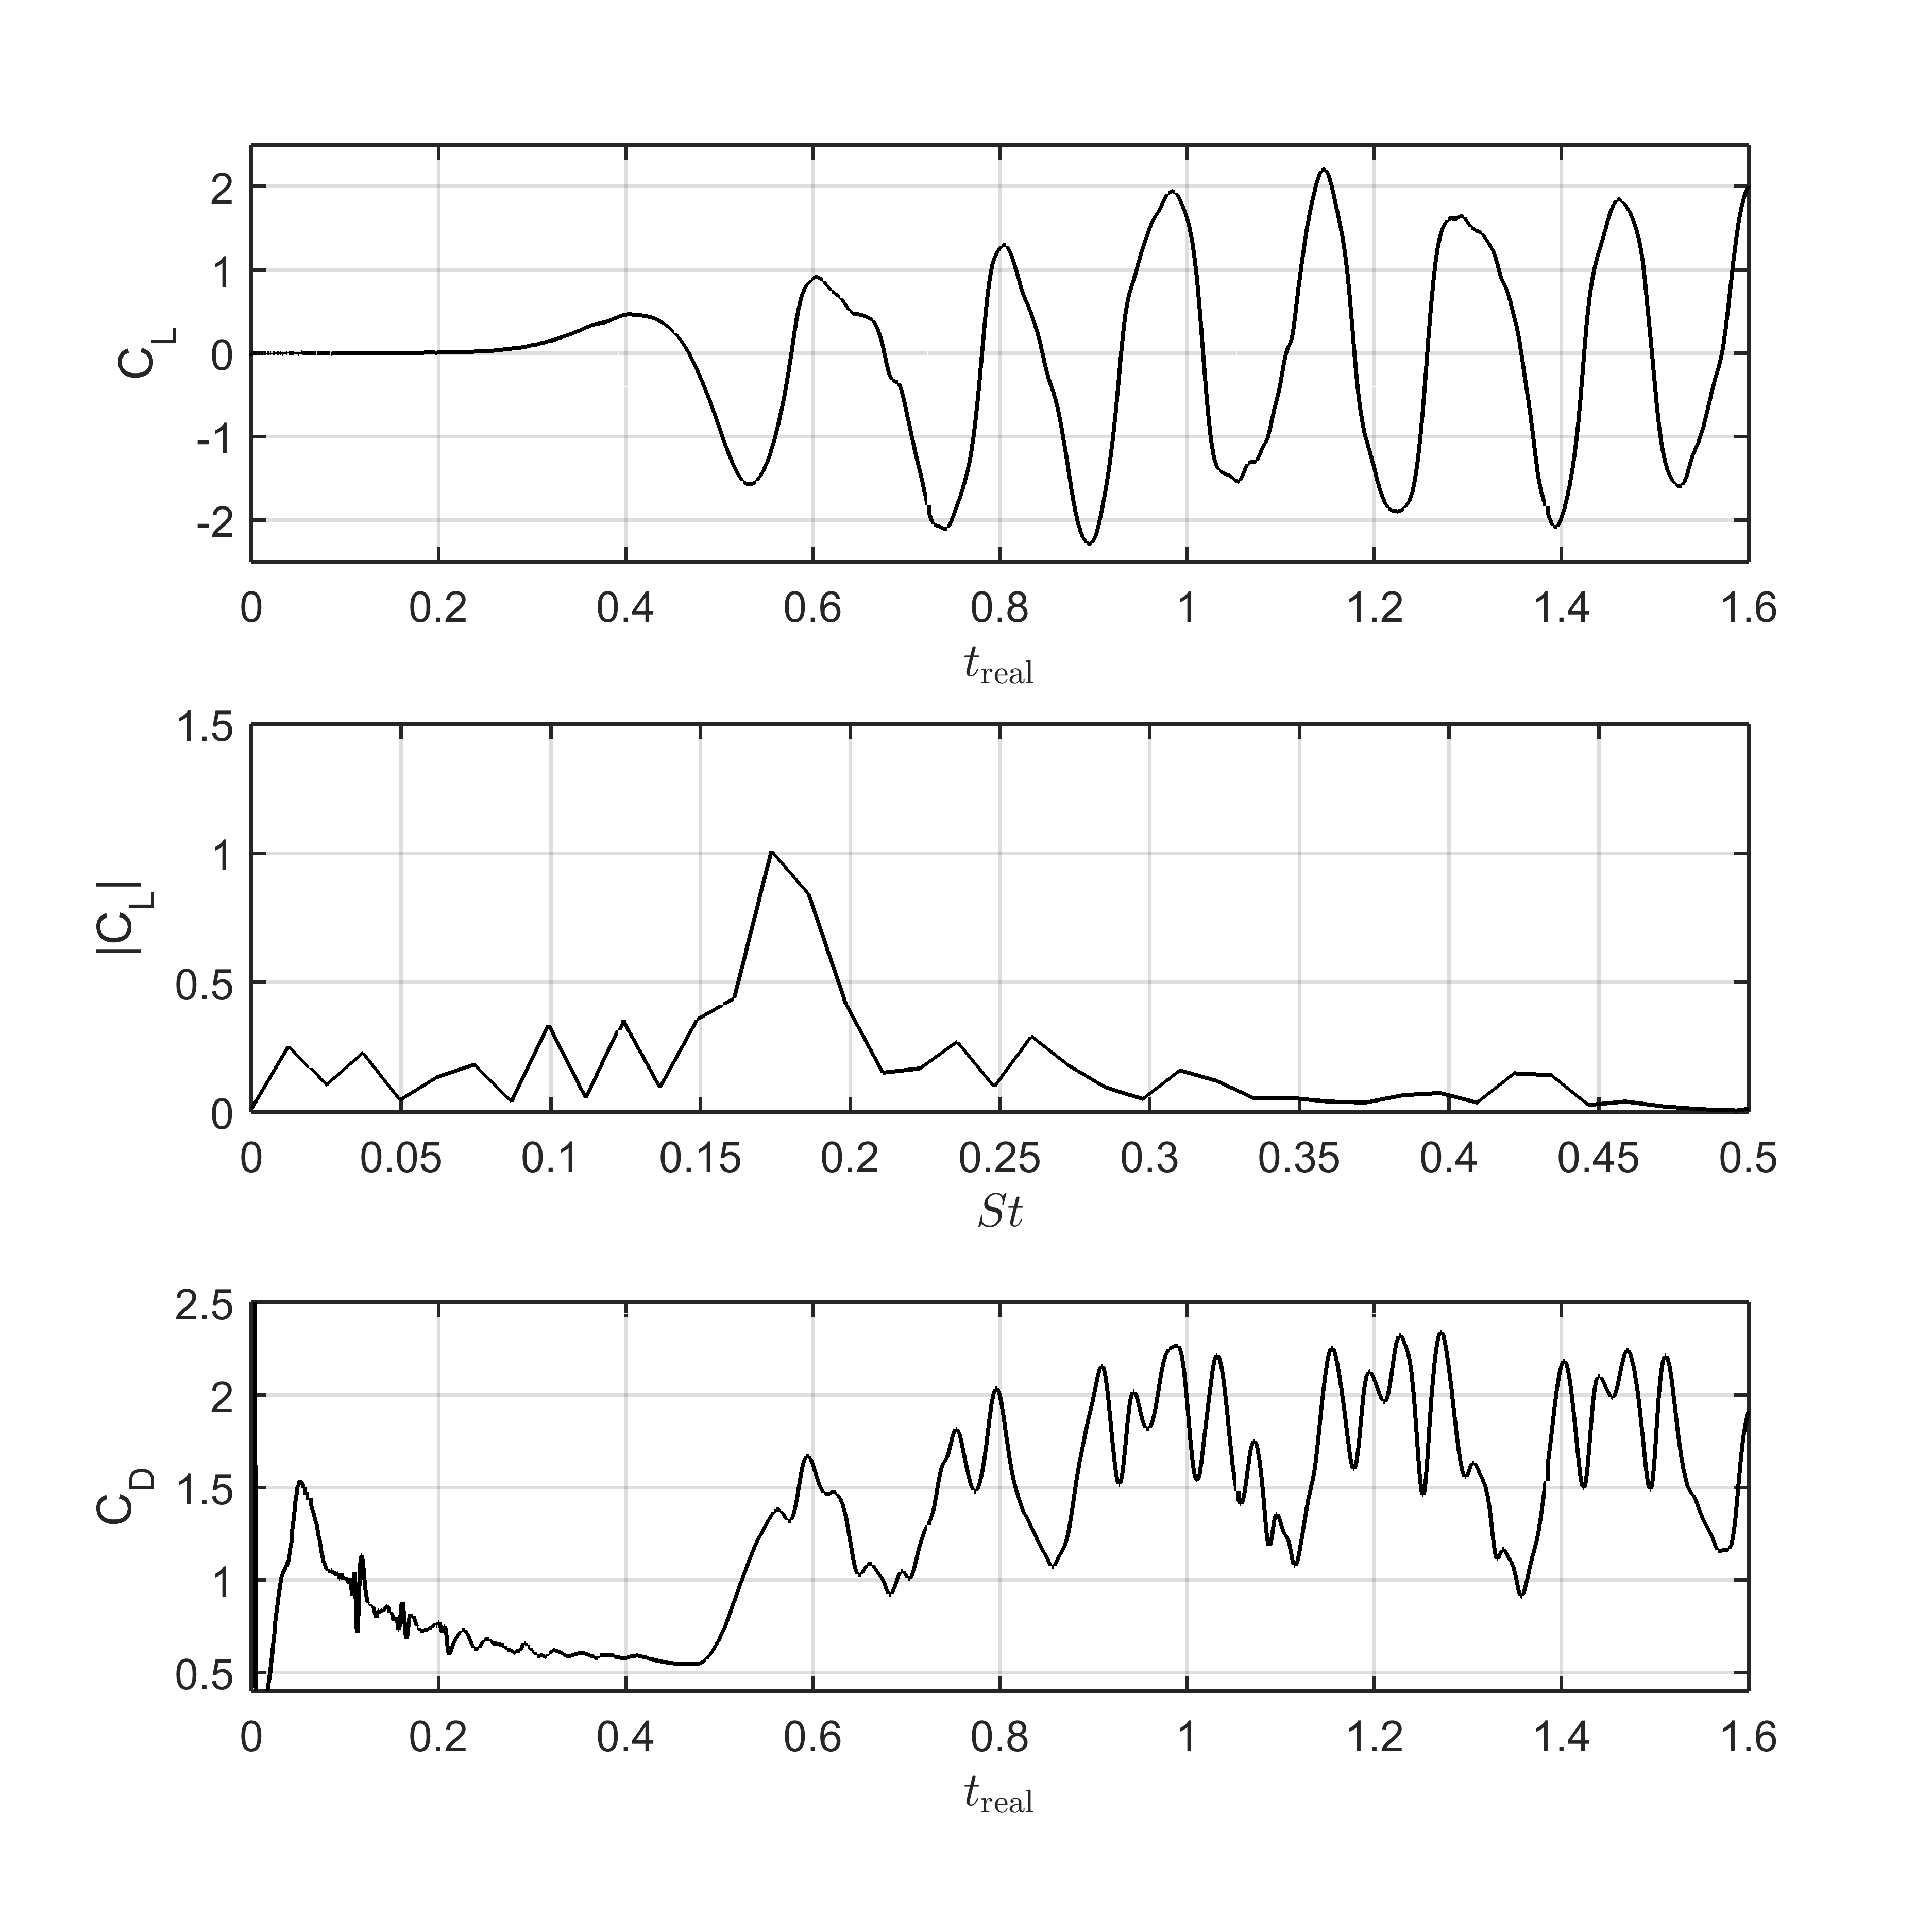
\includegraphics[width = 1\textwidth]{\lfsdir/figs/history_P4_noFilt_mesh4.png}
\caption{Case B in Table \ref{table:filteringEffect_simSummary} lift coefficient, \gls{st} power spectrum, and drag coefficient. Case is not filtered and uses mesh \ref{fig:mesh_case_BDG} with $P=4$.} 
\label{fig:history_P4_noFilt_mesh4}
\end{figure}

\begin{figure}
\centering
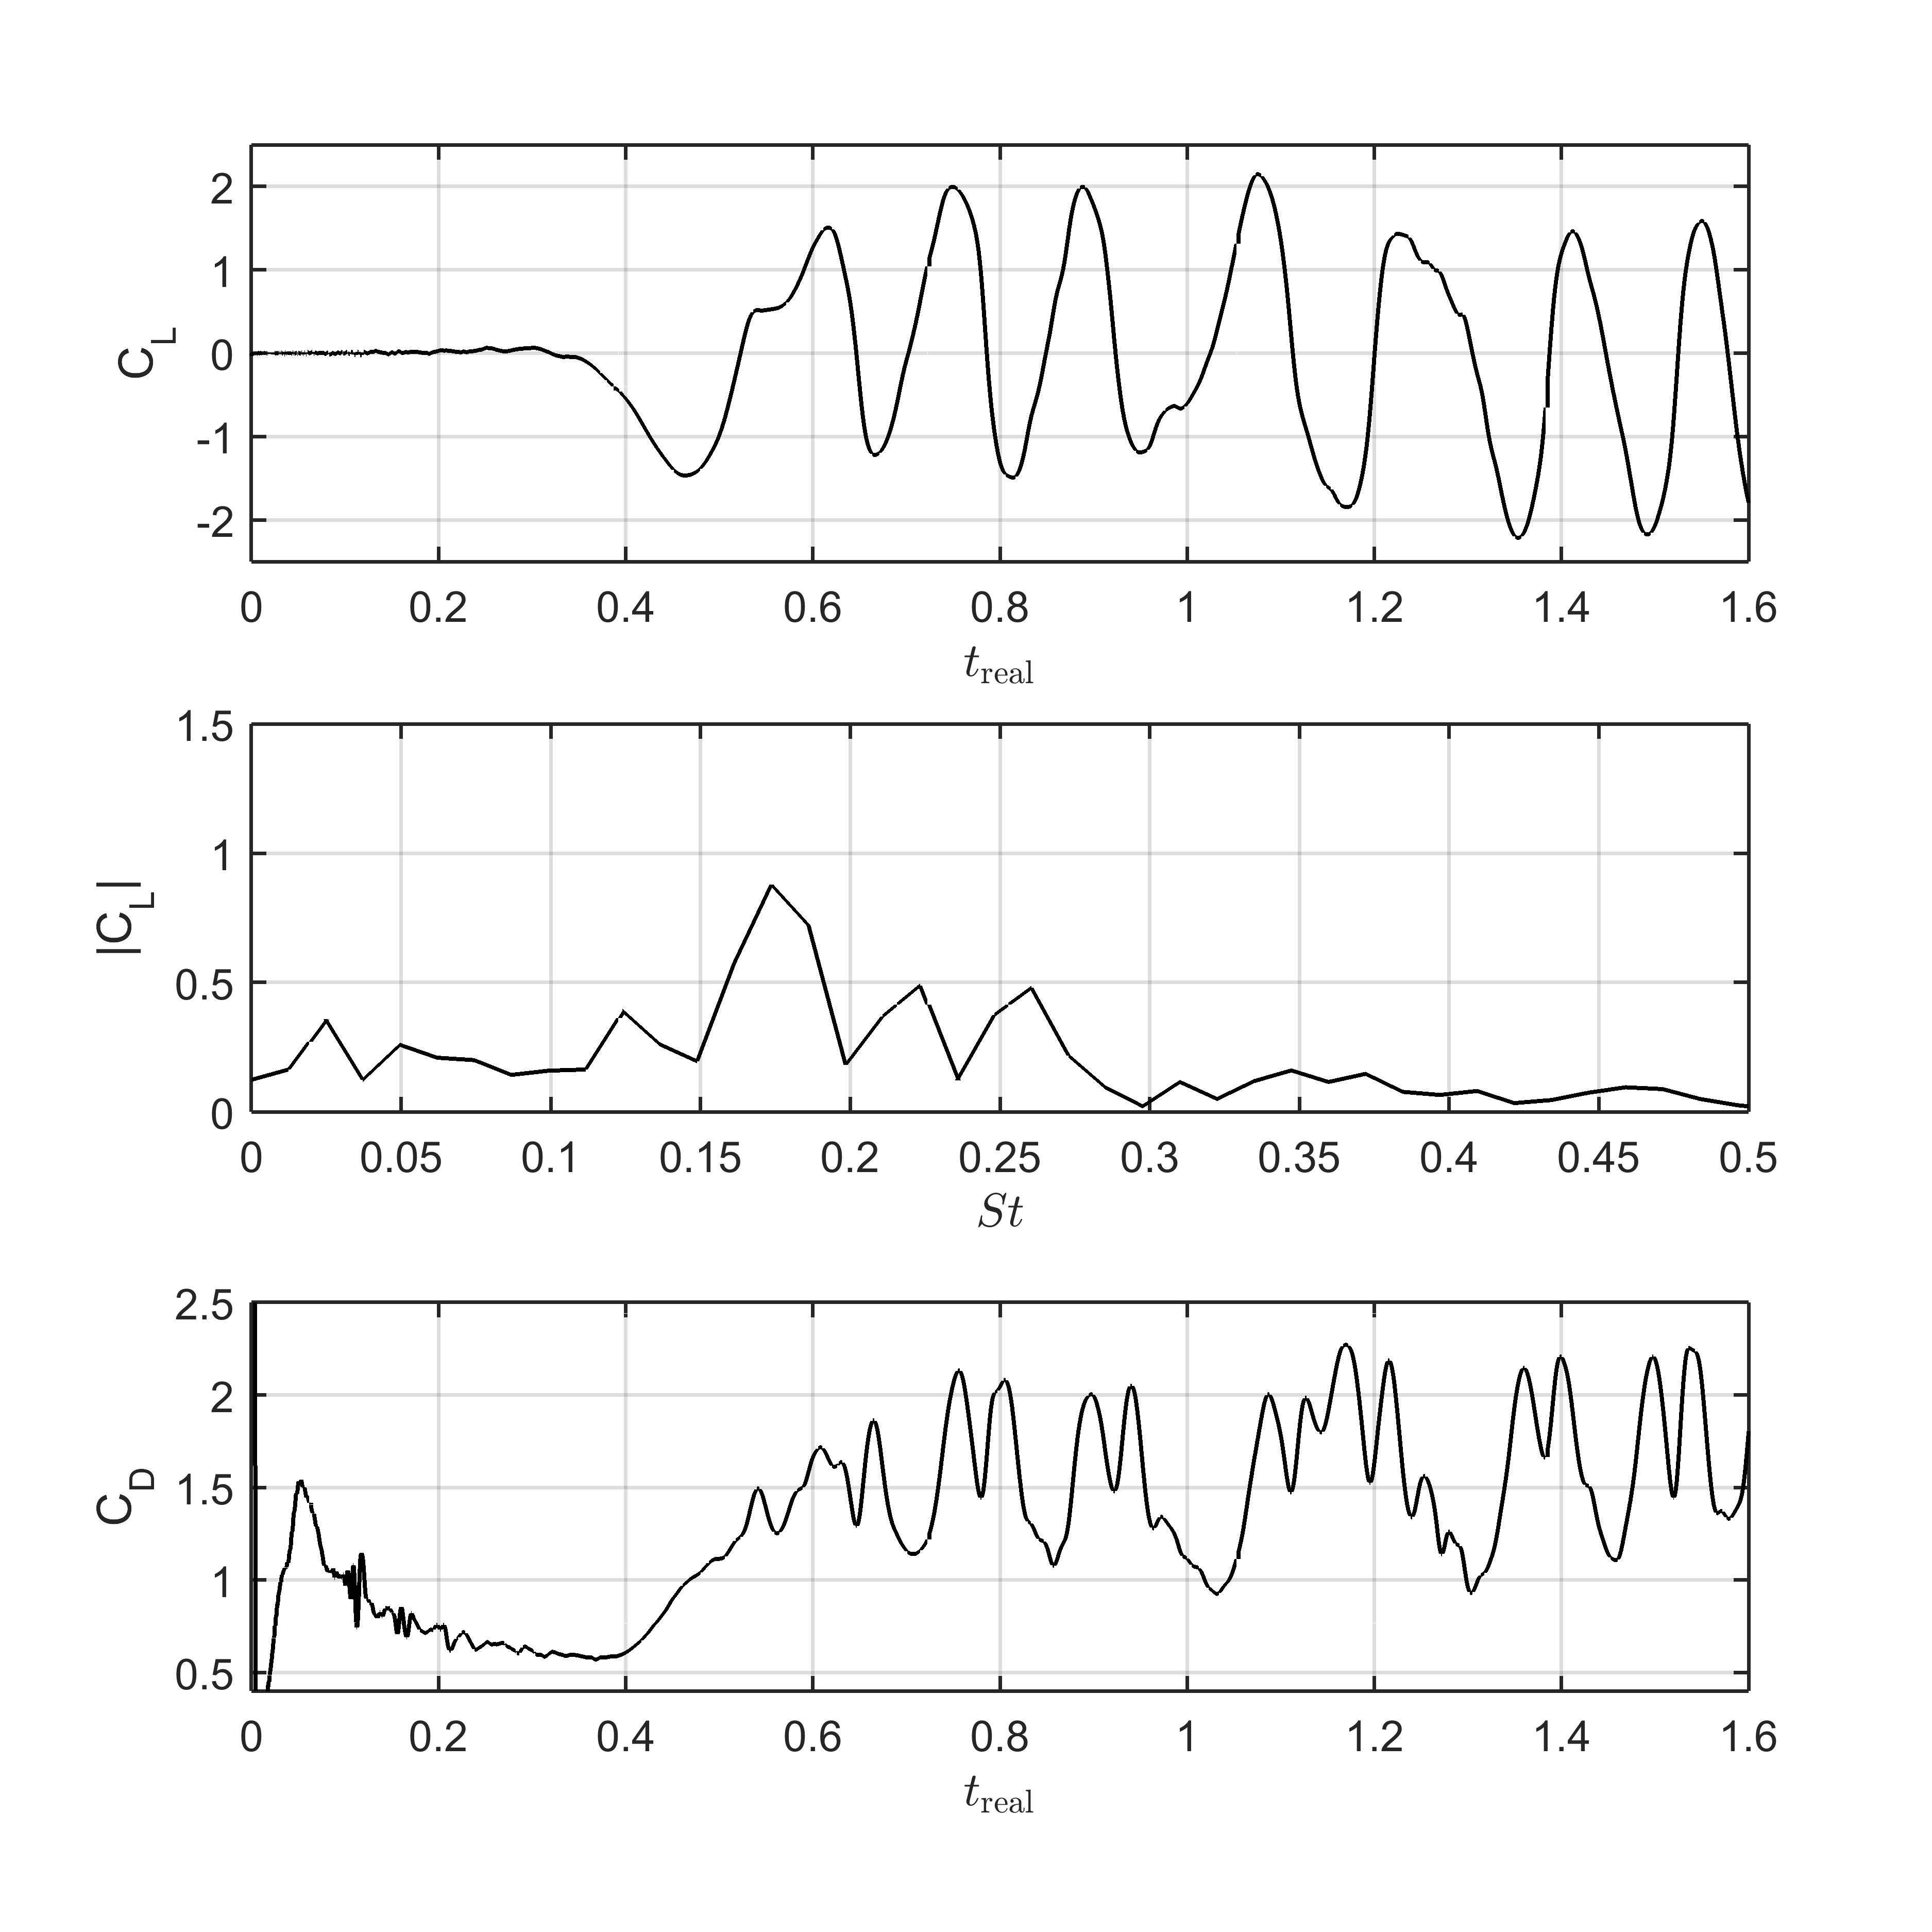
\includegraphics[width = 1\textwidth]{\lfsdir/figs/history_P4_noFilt_mesh6.png}
\caption{Case C in Table \ref{table:filteringEffect_simSummary} lift coefficient, \gls{st} power spectrum, and drag coefficient. Case is not filtered and uses mesh \ref{fig:mesh_case_C} with $P=4$.} 
\label{fig:history_P4_noFilt_mesh6}
\end{figure}

\begin{figure}
\centering
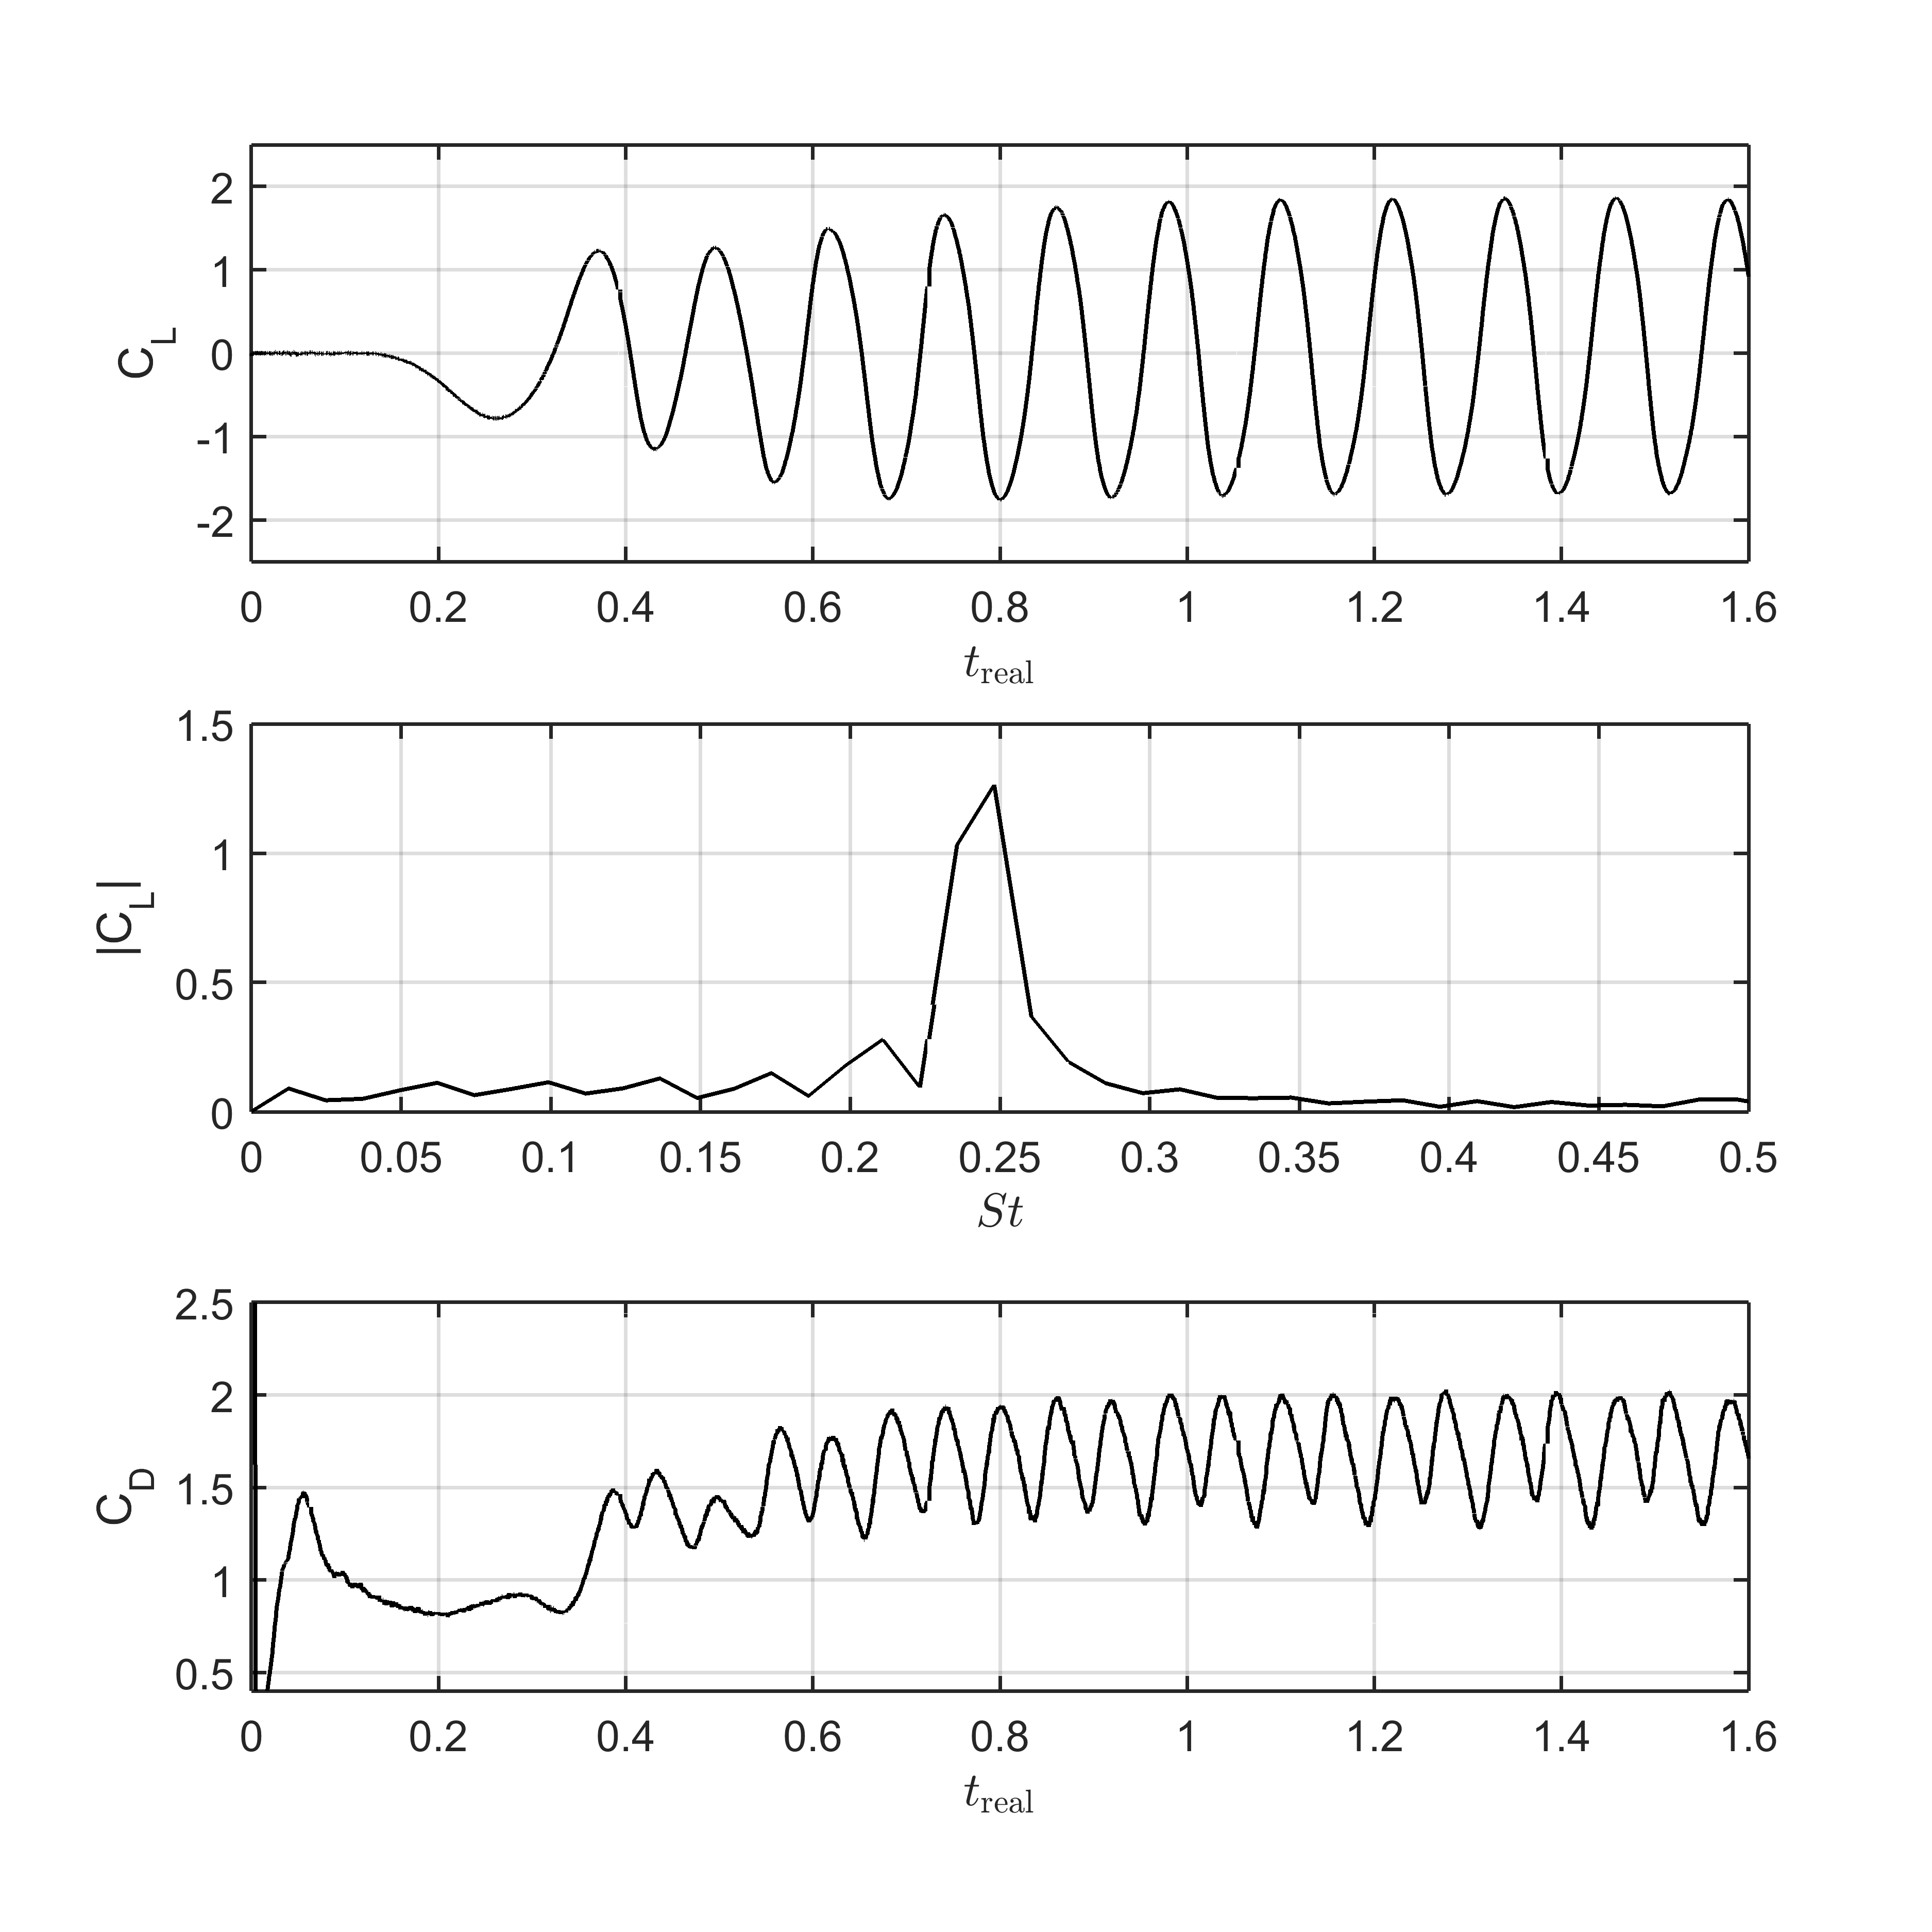
\includegraphics[width = 1\textwidth]{\lfsdir/figs/history_P4_filt_mesh4.png}
\caption{Case D in Table \ref{table:filteringEffect_simSummary} lift coefficient, \gls{st} power spectrum, and drag coefficient. Case is filtered and uses mesh \ref{fig:mesh_case_BDG} with $P=4$.} 
\label{fig:history_P4_filt_mesh4}
\end{figure}

\begin{figure}
\centering
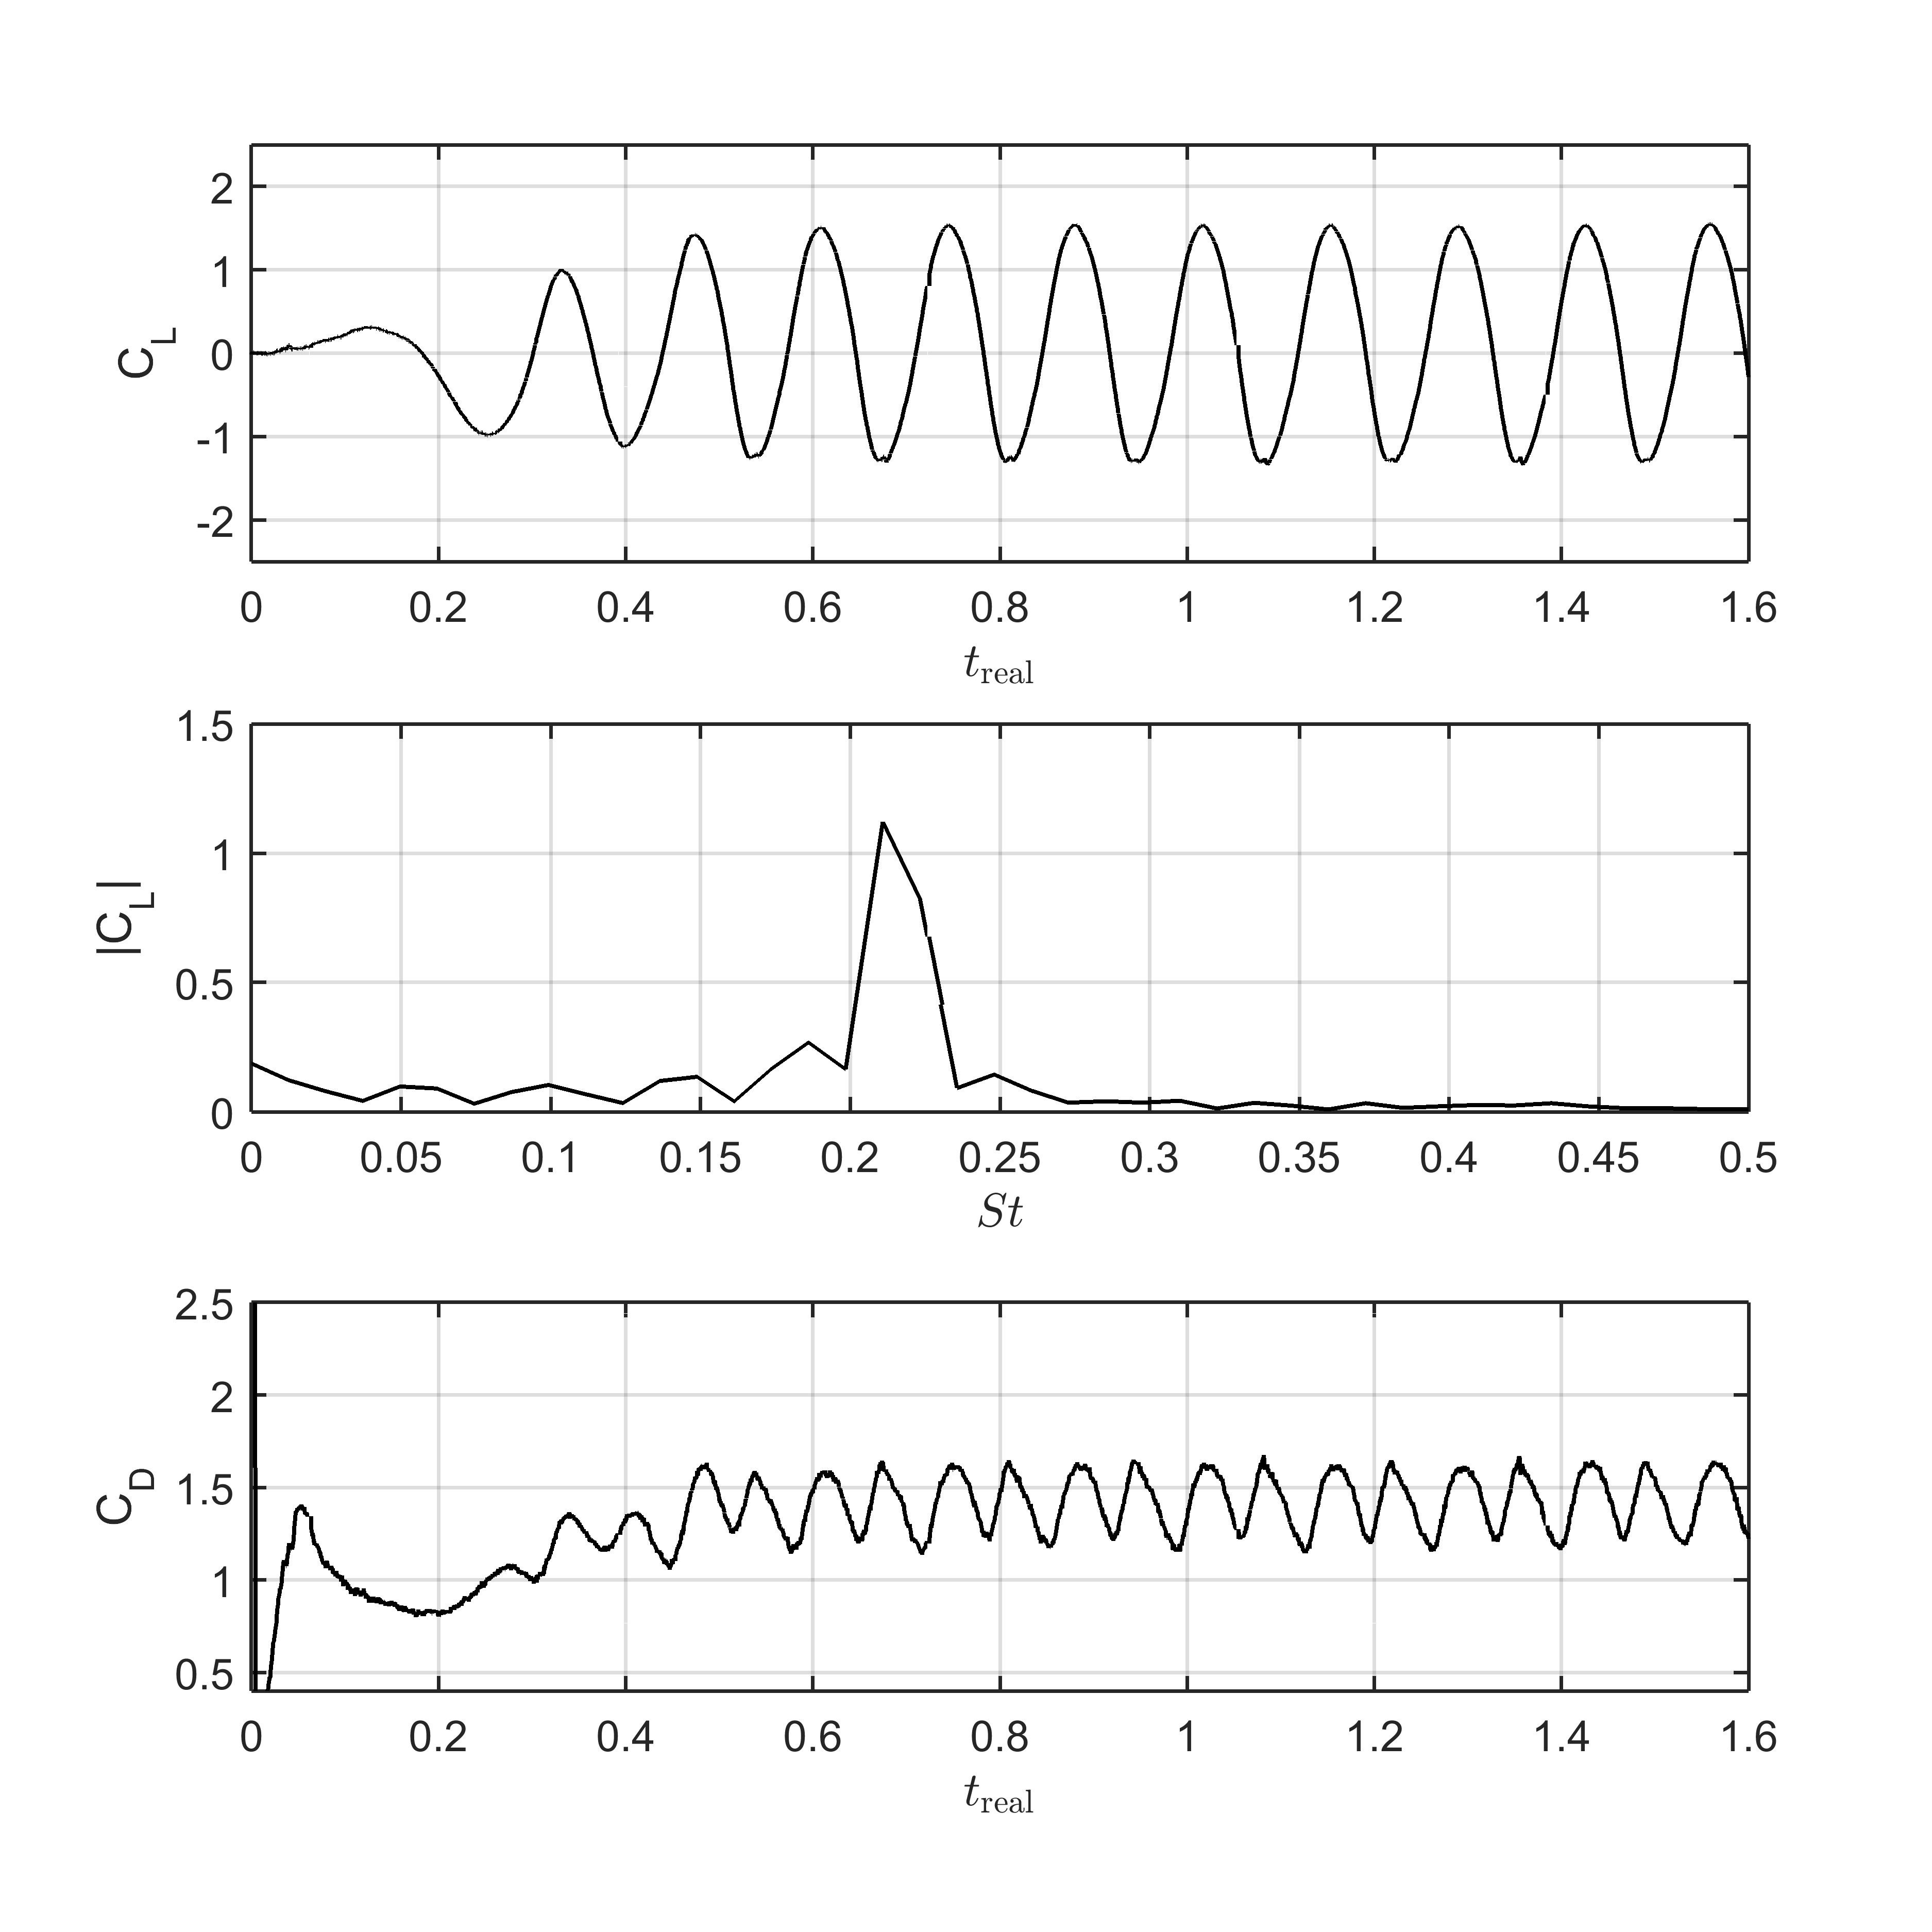
\includegraphics[width = 1\textwidth]{\lfsdir/figs/history_P5_filt_mesh5.png}
\caption{Case F in Table \ref{table:filteringEffect_simSummary} lift coefficient, \gls{st} power spectrum, and drag coefficient. Case is filtered and uses mesh \ref{fig:mesh_case_EF} with $P=5$.} 
\label{fig:history_P5_filt_mesh5}
\end{figure}

\begin{figure}
\centering
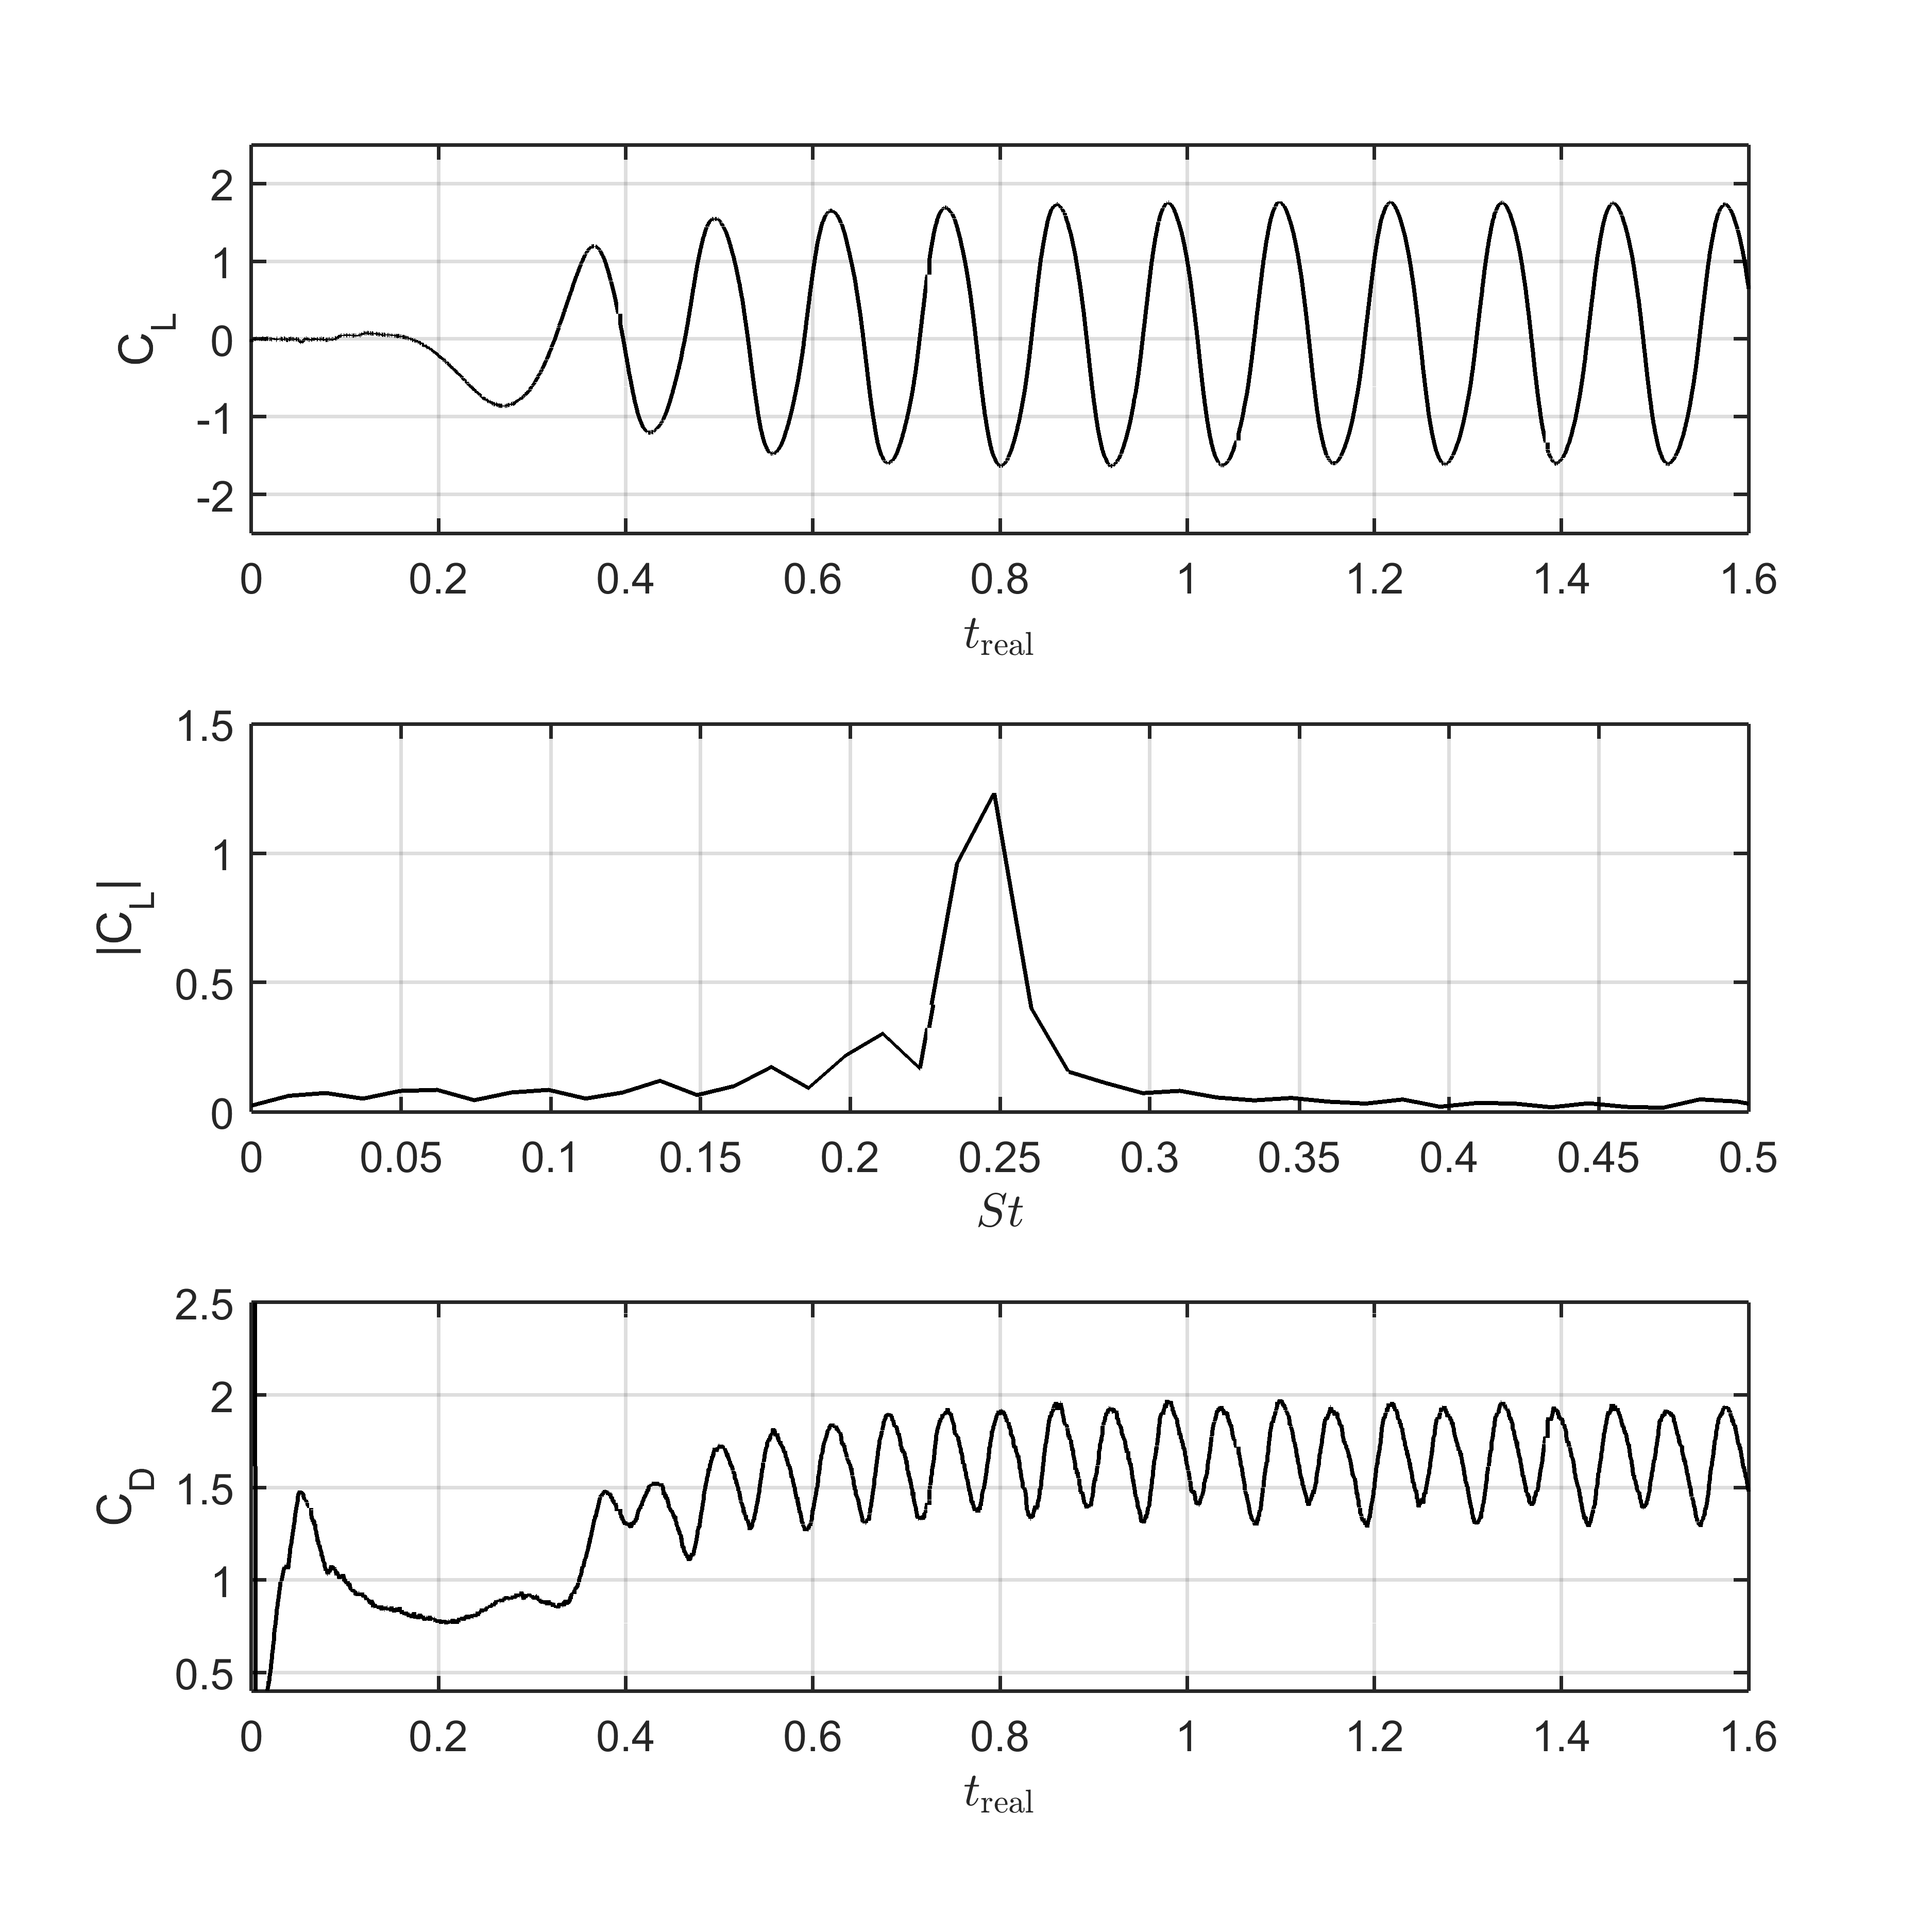
\includegraphics[width = 1\textwidth]{\lfsdir/figs/history_P5_filt_mesh4.png}
\caption{Case G in Table \ref{table:filteringEffect_simSummary} lift coefficient, \gls{st} power spectrum, and drag coefficient. Case is filtered and uses mesh \ref{fig:mesh_case_BDG} with $P=5$.} 
\label{fig:history_P5_filt_mesh4}
\end{figure}

\emph{Effect of changing the spatial order of accuracy while keeping the number of \gls{dof} constant.} Cases \hyperlink{caseA}{A} ($P=1$) and \hyperlink{caseB}{B} ($P=4$) keep close to the same number of \gls{dof}. Their lift coefficient power spectra show that the main vortex shedding frequencies are similar. Their drag coefficient figures reveal that \hyperlink{caseB}{Case B}, as expected, experiences less numerical dissipation; the initial vortices detach later than in \hyperlink{caseA}{Case A}. In addition, the drag coefficient plot in \hyperlink{caseB}{Case B} shows the presence of fairly small structures. \hyperlink{caseA}{Case A} seems to diffuse such structures. This effect can be seen in the corresponding videos as well.

\emph{Effect of changing the number of \gls{dof} while maintaining the spatial order of accuracy constant.} Cases \hyperlink{caseB}{B} and \hyperlink{caseC}{C} differ only in the mesh, \hyperlink{caseC}{Case C} has about half as many \gls{dof} as \hyperlink{caseB}{B}. Both cases have a peak in the lift coefficient power spectrum at \gls{st}$=0.17$. As can be seen in the videos and the drag coefficient plots, smaller structures are present in \hyperlink{caseB}{Case B}, however, \hyperlink{caseC}{Case C} still captures smaller structures than \hyperlink{caseA}{A} ($P=1$) while using half as many \gls{dof} and introduces less dissipation as demonstrated by \hyperlink{caseC}{Case C}'s delayed start of vortex shedding. The strength of the peak at \gls{st}$=0.17$ has decreased in \hyperlink{caseC}{Case C}. This points to the fact that higher dissipation increases the strength of shearing forces on the vortices, thus prompting earlier detachment and smaller lift coefficient oscillation amplitude.

\emph{Effect of using \gls{lfs} filters.}  Cases \hyperlink{caseB}{B} and \hyperlink{caseD}{D} differ only in the filtering. \hyperlink{caseD}{Case D} is filtered. The most salient effect of filtering is that the filtered solution starts shedding vortices earlier, sheds vortices periodically (as opposed to quasiperiodically), and very fine structures are almost non-existent. Indeed the flow looks like the case of \gls{re}$=100$ in Figure \ref{cylinder_3}, yet it predicts a higher mean drag coefficient. The power spectrum of the lift coefficient has very little energy at high values of \gls{st}. This is consistent with the desire of filtering specific frequencies from the simulation. Unfortunately the author could not find studies performed regarding the effect of artificial viscosity on the properties of chaotic flows. Nevertheless, the behavior observed in the filtered solution is consistent with what would be expected of a more viscous flow.

\emph{Effect of spatial order of accuracy on filtered simulations.} Cases \hyperlink{caseD}{D} and \hyperlink{caseG}{G} are both filtered and differ only in the spatial order of accuracy. The two simulations are nearly identical. This result is very encouraging: the filtering formulation maintains the spectral properties independent of the spatial order of accuracy. Recall that the filtering matrices are different for the different schemes. This means that the \gls{lfs} filters' spectral properties can be relied on when developing or using \gls{sgs} models.

\emph{Effect of the mesh on filtered simulations.} Cases \hyperlink{caseF}{F} and \hyperlink{caseG}{G} are both filtered and differ only in the mesh used. The peak \gls{st} number for the coarser grid, \hyperlink{caseF}{Case F}, is lower and its predicted average drag coefficient is lower. This result reflects the general high dependence of simulation results on the grid quality. The grid used in \hyperlink{caseF}{Case F} could not produce a stable unfiltered simulation result even with smaller time-steps. It is possible the shift in the drag coefficient is a reflection of the mesh's improper resolution. This shows that the \gls{lfs} filters could in some cases provide stability at the expense of accurate physics and confirms that \gls{lfs} filters de-couple stability from proper resolution.



% % % % % % % % % % % % % % % % % % % %  Conclusion
\subsubsection{Conclusion}
\label{sec:filterEffectsConclusion}
In the simulations summarized in Table \ref{table:filteringEffect_simSummary}, it was possible to isolate the effects of filtering on a \gls{re}$=3.9e3$, \gls{ma}$=0.1$ 2-D flow past a circular cylinder. The unfiltered solutions in different grids obtained with different spatial orders of accuracy displayed minor differences: all unfiltered flows showed quasiperiodic flow with a peak lift coefficient power at a frequency of \gls{st}$\approx 0.18$. All filtered solutions exhibited an apparent regime change: the flow became periodic and the peak lift coefficient power occurred at a higher frequency.

It could be surmised that the \gls{lfs} filters showed the following strengths:
\begin{enumerate}
\item The scales filtered by \gls{lfs} filters are relative to the element size and virtually independent of the order of the basis polynomials, this could be leveraged in the development of \gls{sgs} models. This was demonstrated by the extremely similar results of Cases \hyperlink{caseD}{D} and \hyperlink{caseG}{G}, which were performed in the same grid with different orders of accuracy.
\item \gls{lfs} filters de-couple stability from proper simulation resolution. This could be very helpful when performing \gls{les} of turbulent flows. If proper resolution were required for stability, such cases would need to have a resolution close to that of \gls{dns}.
\end{enumerate}

The following was identified as a potential drawback:
\begin{enumerate}
\item Application of \gls{lfs} filters in the entirety of the simulation can cause an artificial regime change consistent with what would be expected of increasing viscosity in the flow. This calls for a selective application of \gls{lfs} filters.
\item Because the spectral properties of \gls{lfs} filters scale with the element size, results of flows filtered throughout are grid dependent. Once again, the use of sensors could ameliorate this grid dependence.
\end{enumerate}
